\begin{tikzpicture}
  \tikzset{et/.style={above,font=\footnotesize\vphantom{Ag}}}
  % 
  \node[inner sep=0pt, anchor=south west] (image) at (0,0){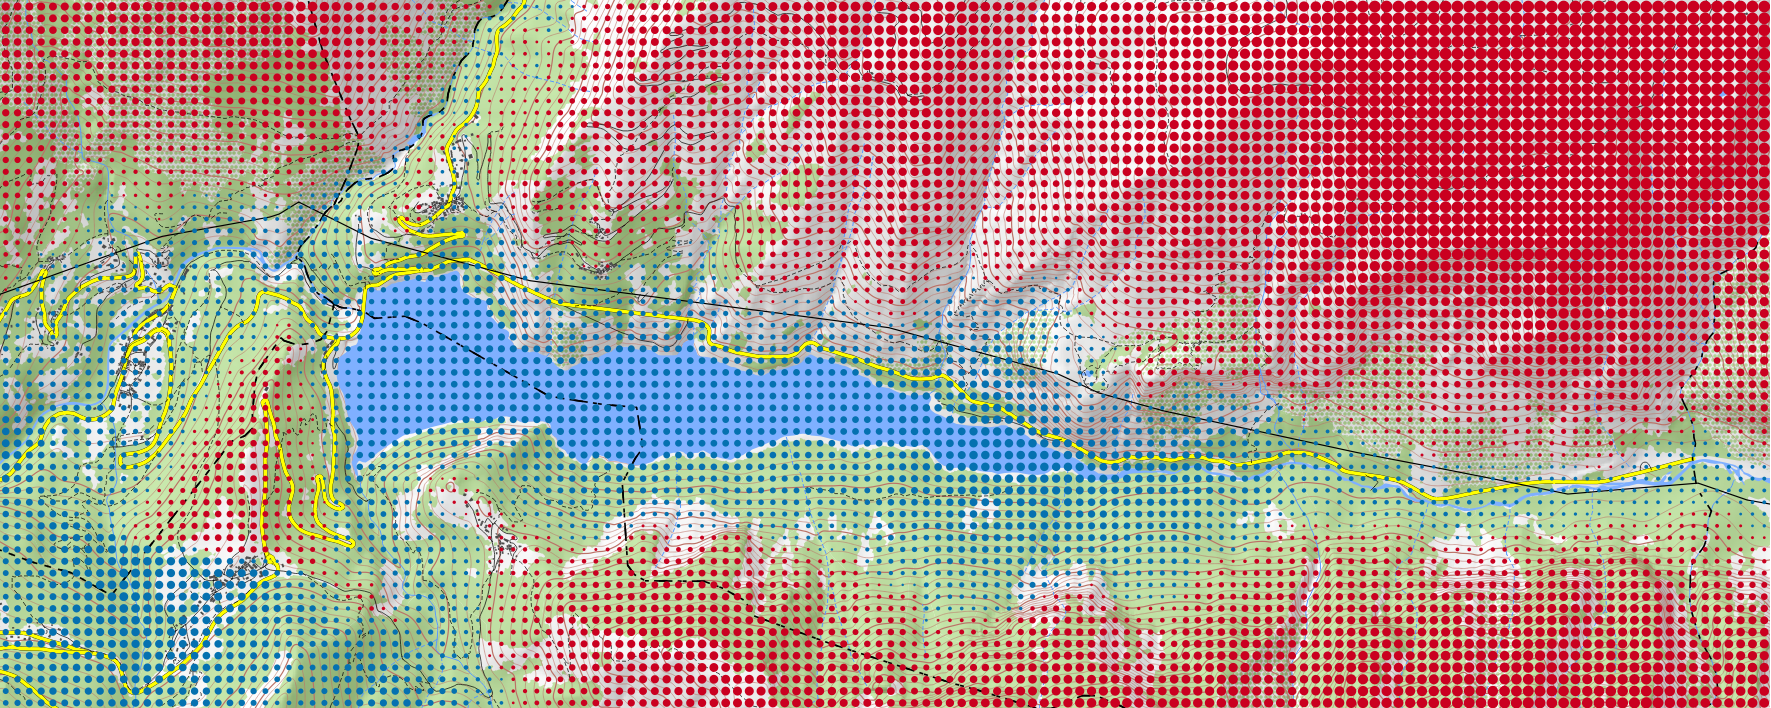
\includegraphics{./figures/Raster_ISO_DALT_HT.png}};
  % 
  \begin{scope}
    \node (P2) at ([yshift=-.5cm]image.south east) {};
    \node (P1) at ([yshift=-.5cm]image.south west) {};

    \node (rect) [anchor=north west, minimum width=1cm,minimum
    height=.25cm] at ([yshift=-.25cm]P1) {}; \path[draw=RdBu-9-1, line
    width=.4mm](rect.west) --([xshift=-1ex]rect.south) -- ([xshift=1ex]rect.north)
    -- (rect.east);
    \node[anchor=west, font=\tiny\vphantom{Ag}, text width = 4cm] at
    ([xshift=1ex]rect.east) {Ligne électrique utilisée comme
      \emph{objet de référence}};
    %
    \node[anchor=west, font=\footnotesize\vphantom{Ag}, text width=8cm] at
    (P1 |- 0cm,-1.85cm) {Différence d'altitude avec la ligne électrique};
    %
    \begin{scope}
      \foreach \x [evaluate=\xshift using 2.5+\x/10, evaluate=\rad using (\x * -.0008) + .05] in {0,...,50}
      {
        \draw[fill=RdBu-9-9,draw=none, below] ([xshift=\xshift cm, yshift=-2.5cm]P1) circle [radius=\rad cm];
      }
      \foreach \x [evaluate=\xshift using 7.5+\x/10, evaluate=\rad using (\x * .0008) + .01] in {0,...,50}
      {
        \draw[fill=RdBu-9-1,draw=none, below] ([xshift=\xshift cm, yshift=-2.5cm]P1) circle [radius=\rad cm];
      }
      % 
      \path(2.5,-3) --++ (10,0)
      node[et,pos=0] {$<$ \SI{-500}{\meter}}
      node[et,pos=.5] {\SI{0}{\meter}}
      node[et,pos=1] {$>$ \SI{500}{\meter}};
    \end{scope}
    
    % \node (rect2) [anchor=north west, minimum width=1cm,minimum
    % height=.25cm] at ([xshift=5.5cm,yshift=-.25cm]P1) {};
    % \path[draw=RdBu-9-9, line width=.25mm](rect2.west)
    % --([xshift=-1ex]rect2.north) -- ([xshift=1ex]rect2.south) --
    % (rect2.east); \node[anchor=west, font=\tiny\vphantom{Ag}, text
    % width = 4cm] at ([xshift=1ex]rect2.east) {Isolignes d'éloignement
    % à \emph{l'objet de référence} (équidistance \SI{250}{\meter})};

    % Échelle
    \draw[-] (P2 |- -1cm,-1cm) --++ (-1,0) node[et,pos=.5] {\SI{500}{\meter}};
    % Légende détaillée
    \path (P1) -- (P2) node[pos=.5, yshift=-3cm] {\tiny Pour la
      légende détaillée du fond topographique voir
      \autoref{anx:topo_leg}. Sources: BD TOPO 2018, BD ALTI 2018.};
  \end{scope}
\end{tikzpicture}